\subsection{داده افزایی}\label{subsec:داده-افزایی}

داده افزایی یکی از پیش‌پردازش‌هایی ست که قبل از داده شدن داده‌ها به مدل، روی آن‌ها انجام می‌شود.
در داده افزایی\LTRfootnote{Data Augmentation} از تصاویر موجود، تصاویر جدیدی بازآفرینی می‌شوند.
معمولا تصاویر جدید ایجاد شده، توزیع داده نزدیکی به توزیع داده ی داده‌های اصلی و تست دارند و هدف از این کار این است که تعمیم یافتگی مدل را افزایش دهیم تا دقت مدل بر روی داده‌های تست افزایش پیدا کند.
روش‌ها و الگوریتم‌های مختلف با پیچیدگی‌های مختلفی وجود دارد که در ادامه روش‌هایی که در این پروژه مورد بررسی قرار گرفت، آمده است.
\subsubsection{چرخش تصویر به صورت تصادفی}
در این روش تصاویر به اندازه مقداری تصادفی چرخ داده می‌شوند\LTRfootnote{Random Rotate}.
از آنجایی که در این مسئله، با چرخش، تصاویر اطلاعاتی از دست نمی دهند و علاوه بر آن، مقدار خروجی مدل ما نیز نباید تغییر کند، لذا می‌توان از این روش برای داده افزایی استفاده کرد.

\subsubsection{آینه کردن به صورت تصادفی}
مانند قسمت قبل،از این روش نیز می‌توان برای داده افزایی استفاده کرد\LTRfootnote{Random Flip}.

\subsubsection{تغییر مقیاس به صورت تصادفی}
معمولا عکس‌هایی که از آن‌ها برای آموزش مدل استفاده می‌کنیم دارای ابعاد و رزولوشن متفاوتی هستند و در نتیجه اندازه سلول‌ها در آن‌ها متفاوت است.
از آنجایی که مدل در نهات تلاش می‌کند ویژگی‌های مرتبط با این سلول‌ها را بیابد و با توجه به آن‌ها، تشخیص درستی را ارایه دهد، باید پیش‌پردازشی انجام گیرد تا مدل نسبت به اندازه سلول‌ها، حساس نشود. از این روی می‌توان قبل از استفاده از عکس‌ها در آموزش مدل، مقیاس تصاویر را به صورت تصادفی تغییر داد\LTRfootnote{Random Scale}.

\subsubsection{بلور کردن به صورت تصادفی و اضافه کردن نویز گوسین }
ممکن است تصاویر اسکن شده، به خوبی تصاویر زمان آموزش مدل نباشد و عوامل محیطی، باعث بوجود آمدن نویز در داده‌ها شده باشد، از این روی ما از قصد نویز و یا بلور رو به عکس زمان آموزش اضافه می‌کنیم تا مدل توانایی بیشتری برای پیشبینی درست روی عکس‌های نویزی داشته باشد.

\subsubsection{تغییر رنگ}
همانطور که پیشتر نیز گفته شد، عکس‌ها و اسلاید‌ها ممکن است با روش‌های متفاوتی رنگ شده باشند و رنگ‌های مختلفی را به خود بگیرند.
از این روی باید عکس‌های زمان آموزش مدل نیز به اندازه کافی تنوع رنگ داشته باشد و مدل توانایی تشخیص درست در بازه رنگ‌های متفاوتی را داشته باشد.
برای این کار می‌توان عکس‌ها را قبل از داده شدن به مدل تغییر داد تا رنگ‌های آن‌ها تغییر کند.
روشی که در این جا استفاده می‌شود به این صورت است که در ابتدا عکس‌ها را از حالت \lr{RGB} به \lr{HSV} تبدیل می‌کنیم.
در دامنه \lr{HSV}، کانال‌ها به ترتیب حاوی اطلاعات رنگ\LTRfootnote{Hue}، اشباع\LTRfootnote{Saturation} و روشنایی\LTRfootnote{Brightness} هستند.
در اینجا کافیست مقدار کانال رنگ را که مقداری بین 0 تا 360 به خود می‌گیرد را صورت تصادفی تغییر دهیم.
در تصویر \ref{jitter augmentation} مثالی از این پیش‌پردازش آمده است.
\begin{figure}
    \begin{center}
        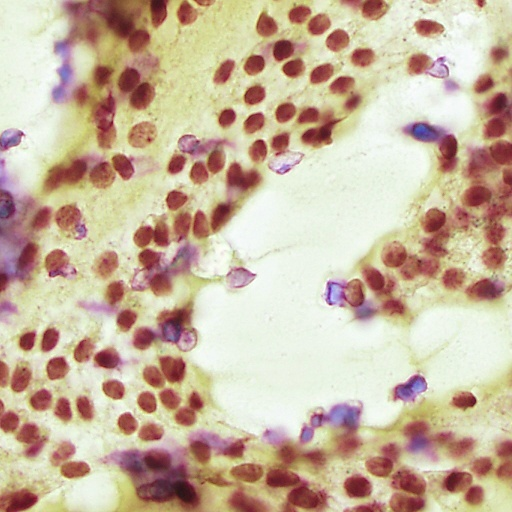
\includegraphics[width=0.48\linewidth]{figs/suggested_methods/subs/data_augmentation/jitter_1054-original.jpeg}
        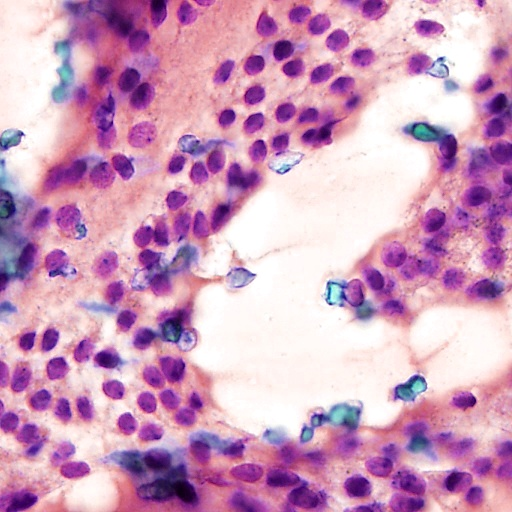
\includegraphics[width=0.48\linewidth]{figs/suggested_methods/subs/data_augmentation/jitter_1054-transformed.jpeg}
    \end{center}
    \caption{نمونه‌ای از پیش‌پردازش تغییر رنگ که به ترتیب از راست به چپ عکس اصلی و عکس تبدیل‌شده را نشان می‌دهد.}
    \label{jitter augmentation}
\end{figure}

\subsubsection{تطبیق دامنه فوریه}
%https://towardsdatascience.com/deep-domain-adaptation-in-computer-vision-8da398d3167f
در هنگام آموزش یک مدل، فرض می‌شود که داده‌های آموزشی شما (چه بزرگ یا کوچک) نماینده خوبی از توزیع کلی داده‌هاست.
با این حال، اگر ورودی‌ها در زمان آزمون به طور قابل توجهی با داده‌های آموزشی متفاوت باشد، مدل ممکن است عملکرد چندان خوبی نداشته باشد در حالی که برای یک انسان، با یادگیری مفهوم یک موضوع این مشکل کمتر وجود دارد.
دلیل اینکه مدل شما در این سناریوها خیلی خوب عمل نمی کند این است که دامنه مسئله تغییر کرده است. در این مورد تطبیق دامنه به کمک شما می‌آید. تطبیق دامنه زیرشاخه‌ای از یادگیری ماشین است که به سناریوهایی می‌پردازد که در آن یک مدل آموزش‌دیده بر روی توزیع منبع در زمینه توزیع هدف متفاوت استفاده می‌شود. به طور کلی، تطبیق دامنه\LTRfootnote{Domain adaptation} از داده‌های برچسب گذاری‌شده در یک یا چند دامنه منبع برای حل وظایف جدید در یک دامنه هدف استفاده می‌کند.
\newline
به طور مثال در مسئله این پروژه تنظیمات دستگاه اسکنر و نوع آن، روش اسکن، روش نمونه برداری و ... ممکن است روی توزیع داده‌ها تاثیر بگذارد در حالی که این عوامل در بیمارستان‌های مختلف و مجموع‌داده‌های مختلف متفاوت است، لذا استفاده از تطبیق دامنه، گزینه خوبی برای افزایش عملکرد مدل است.

یکی از روش‌های تطبیق دامنه، تطبیق دامنه فوریه\LTRfootnote{Fourier domain adaptation} است. این روش ابتدا در سال 2020 میلادی و در مقاله \cite{yang2020fda} معرفی شد و به این صورت عمل می‌کند که ابتدا عکس‌های هدف و منبع را با تبدیل فوریه به حوزه فرکانس می‌برد، سپس ناحیه با فرکانس پایین در داده‌های منبع را با ناحیه‌های هدف جاگزین می‌کند و بعد از آن فوریه معکوس را روی داده‌ها انجام داده و داده‌های به حالت قبل بر می‌گردند. دلیل و انگیزه این روش است که طیف دامنه سطح پایین حوزه فرکانس می‌تواند به طور قابل توجهی تغییر کند بدون اینکه بر درک معناشناسی سطح بالا تأثیر بگذارد و با این تغییر، توزیع تصویر نهایی به تصویر هدف نزدیک می‌شود.
این روش بااینکه هزینه محاسباتی بسیار کمی دارد، اما در مواردی عملکرد خوبی رو ارائه کرده است که نمونه از عملکرد این روش، در تصویر \ref{fda augmentation} آمده است.
\begin{figure}
    \begin{center}
        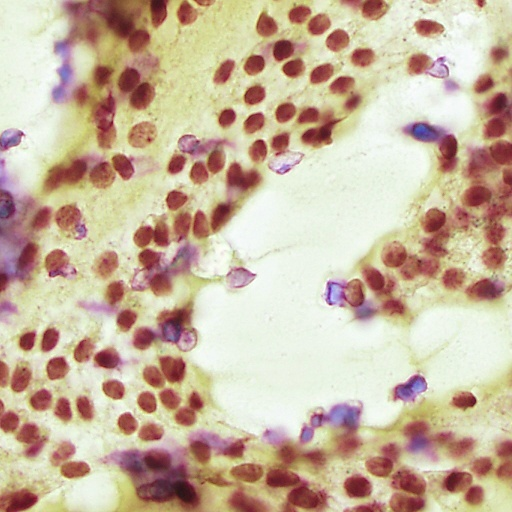
\includegraphics[width=0.48\linewidth]{figs/suggested_methods/subs/data_augmentation/fda_1054-original.jpeg}
        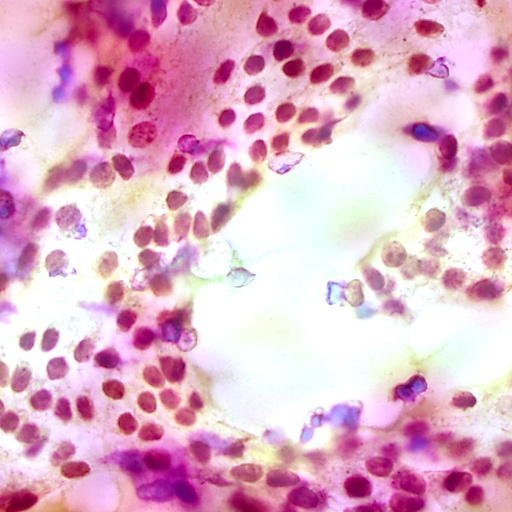
\includegraphics[width=0.48\linewidth]{figs/suggested_methods/subs/data_augmentation/fda_1054-transformed.jpeg}
    \end{center}
    \caption{نمونه‌ای از پیش‌پردازش تطبیق دامنه فوریه که به ترتیب از راست به چپ عکس اصلی و عکس تبدیل‌شده را نشان می‌دهد.}
    \label{fda augmentation}
\end{figure}

\subsubsection{ادغام تصاویر}
ادغام تصویر\LTRfootnote{Mix-up} یکی از روش‌های افزایش داده است که ابتدا در سال 2017 مقاله
\cite{zhang2017mixup}
معرفی شد.
این تکنیک کاملاً سیستماتیک نامگذاری شده است که در آن به معنای واقعی کلمه ویژگی‌ها و برچسب‌های مربوط به آنها را با هم مخلوط می‌کنیم. شبکه‌های عصبی، مستعد به خاطر سپردن برچسب‌های اشتباه هستند. رویه ذکر‌شده این کار را با ترکیب ویژگی‌های مختلف با یکدیگر کاهش می‌دهد (همین مورد برای برچسب‌ها نیز اتفاق می‌افتد) به طوری که یک شبکه در مورد رابطه بین ویژگی‌ها و برچسب‌های آنها بیش از حد مطمئن نشود.
همانطور که گفته شد در ادغام دو عکس را با ضرایب $\lambda$ و ۱-$\lambda$ بین صفر و یک، پیکسل به پیکسل با هم جمع می‌کنند تا عکس جدیدی بدست آید. مقدار $\lambda$ طوری انتخاب می‌شود که تصویر اصلی دچار تغییر معنا نشود.
نمونه‌ای از نتایج این روش در تصویر \ref{mixup augmentation} آمده است.
\begin{figure}
    \begin{center}
        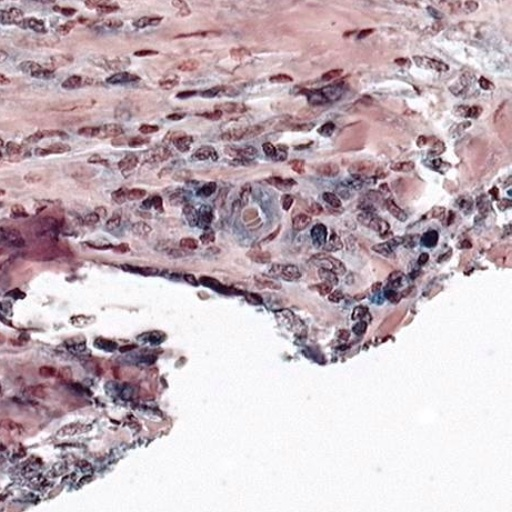
\includegraphics[width=0.48\linewidth]{figs/suggested_methods/subs/data_augmentation/mixup_776-original.jpeg}
        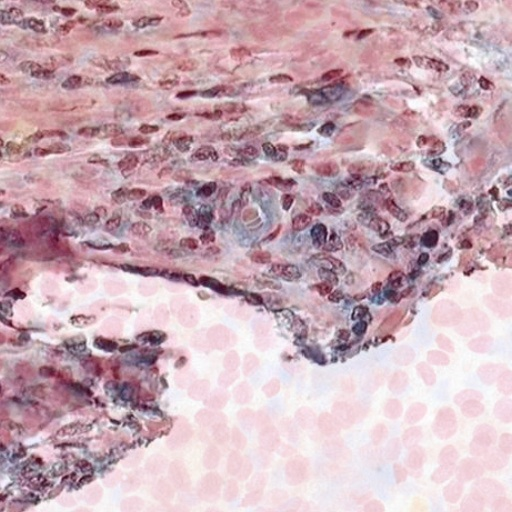
\includegraphics[width=0.48\linewidth]{figs/suggested_methods/subs/data_augmentation/mixup_776-transformed.jpeg}
    \end{center}
    \caption{نمونه‌ای از پیش‌پردازش ادغام تصویر که به ترتیب از راست به چپ عکس اصلی و عکس تبدیل‌شده را نشان می‌دهد.}
    \label{mixup augmentation}
\end{figure}
